\chapter{Methodology / System Implementation}
\label{chap4}


In this chapter we describe the modeling approaches that were used for the creation of the business location recommendation system. We begin by discussing the general motivation behind each method that led to their implementation and comparison, and then proceed to further analyze each in detail.


%==================================================
%==================================================
%==================================================
\section{Overview of Modeling Approaches}

Given the recommandation system we aim to implement, and the ambition to achieve this through the use of generative AI, two state-of-the-art approaches were suggested for the task, each with different strengths, limitations, and ways of utilizing the gathered data. An initial approach involves fine-tuning a Large Language Model (LLM) to specialize in predicting optimal locations while also providing a contextual and user-personalized response. An alternative approach that has emerged in recent years is the construction of a Retrieval-Augmented Generation (RAG) system. In this framework, the actual decision-making process takes place outside the LLM, which is instead used to generate the chatbot-like user output.

Both methodologies present different strengths, limitations and implementation details. In general, a fine-tuned LLM is expected to provide a faster inference that can generalize better on unseen prompts due to its wider knowledge as a pre-trained model. The RAG workflow ,on the other hand, supposedly reduces the hallucinations since its memory does not lie inside the LLM but it fetches data from databases at runtime, and can possibly lead to better personalization due to its more interpretable re-ranking ability. 




%==================================================
%==================================================
%==================================================
\section{Fine-tuned LLM}
\label{sec:fine_tuned_llm}

This section examines the approach of fine-tuning an LLM to specialize on the task of providing the three best locations to open a business. We will first analyze the motivation behind this method, then show the detailed process of creating the fine-tuning and inference datasets, and finally describe the fine-tuning attempts and their comparison based on their results on the inference dataset.


%==================================================
%==================================================
\subsection{Motivation}

Traditional recommendation systems, such as collaborative filtering, content-based filtering, and hybrid approaches, have long been prominent in the field of data science. Despite their indisputable effectiveness, limitations like the cold start problem (struggling when limited historical data is available) or the lack of the explainability of the recommendations have led to the gradual adoption of LLMs in the field. Although several attempts in general recommendation tasks (e.g. movies, products) have tested the suitability and success of LLMs, their application in spatial data and specifically business location recommendation is still very limited. In addition, the potential to provide contextual and personalized suggestions along with justification represents a novel yet promising approach that led to the idea of using LLMs for this problem. In the following paragraph, we show the creation of the essential datasets, the detailed fine-tuning, and the evaluation of the final model. 


%==================================================
%==================================================
\subsection{Fine-Tuning Dataset Creation}
\label{sec:fine_tune_dataset_creation}

This section describes analytically the construction of the fine-tuning dataset. This constitutes the core of the methodology, as the 
content and structure of the final model's outputs are learned directly based on its training data. 


%==================================================
\subsubsection{Synthetic NACE Categories}


The final goal is a model that responds to an every-day description of the business that the user is interested in, ("Where can I open a cafe in Volos?"), not one that specifically mentions its NACE class ("Where can I open a business of NACE class 56.3?"), since this encoding is too technical, or even unknown to the user. Therefore, training prompts should consist of such category descriptions and not the NACE classes themselves. In order to obtain such descriptions generative AI was used. Ιn particular, ChatGPT was produced 3 synthetic categories for each NACE class \ref{fig:synthetic_categories}. Each synthetic category will correspond to 1 entry on the fine-tuning dataset, resulting in 306x3 = 918 entries.

\begin{figure}[!htbp]
    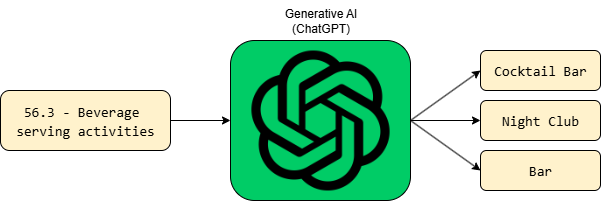
\includegraphics[scale=0.4]{figures/synthetic_categories.png}
    \centering
    \caption{Synthetic Categories Creation}
    \label{fig:synthetic_categories}
\end{figure}


%==================================================
\subsubsection{Feature Importance per NACE Class}

Looking forward, we aim to involve justification for every suggestion provided, as one of the primary motivations of using an LLM was explainability. Since the features describe various aspects of the suggestion (e.g. distance from city center, distance from main roads, area), we aim to use their values for the appropriateness of the recommendation. This requires deciding which features to include in the model's response, since using them all would generate unnecessarily long outputs. To make this decision, feature importance was found and used as a ranking criterion to select features from highest to lowest. The ranking was found individually for every NACE class, since it is assumed that feature importances change between different business types. To acquire the feature importances per NACE class, I used the 'shap' library.


\begin{figure}[h]
    \centering
    \begin{minipage}[b]{0.45\textwidth}
        \centering
        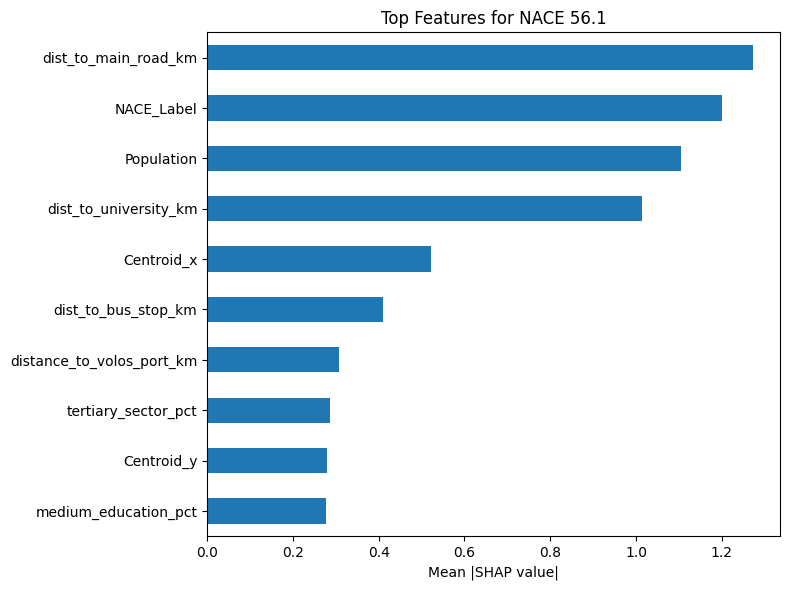
\includegraphics[height=5cm]{figures/shap_56_10.png}
        \caption{SHAP Values of NACE Class 56.10}
        \label{fig:shap_56_10}
    \end{minipage}
    \hfill
    \begin{minipage}[b]{0.45\textwidth}
        \centering
        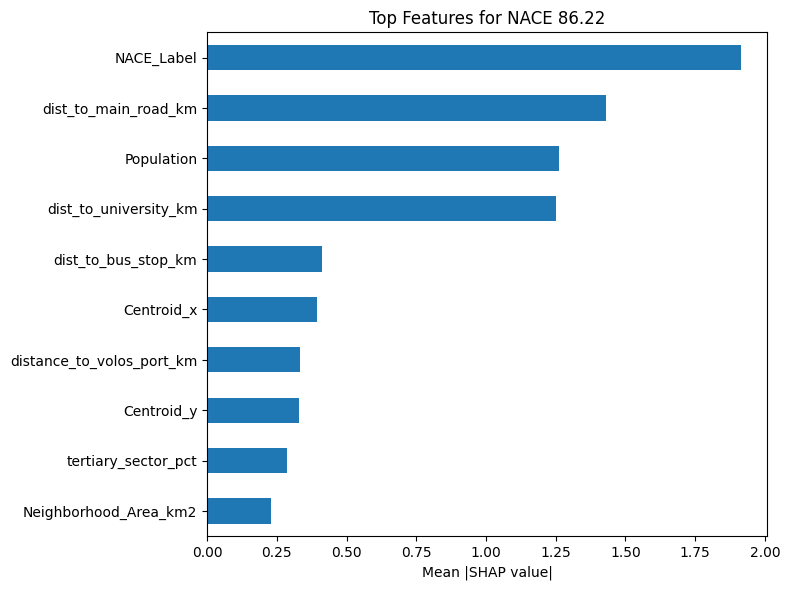
\includegraphics[height=5cm]{figures/shap_86_22.png}
        \caption{SHAP Values of NACE Class 86.22}
        \label{fig:shap_86_22}
    \end{minipage}
\end{figure}

An XGBoost machine learning model was trained on a dataset consistsing of all possible (NACE Class, Neighborhood) pairs, resulting in 306 x 48 = 14.688 entries. Each entry is joined with its corresponding neighborhood and municipal community features (apart from 'Neighborhood\_Greek', 'Geometry' and 'ΠΕΡΙΦΕΡΕΙΑΚΗ ΕΝΟΤΗΤΑ', 'ΔΗΜΟΣ', 'ΔΗΜΟΤΙΚΗ ΕΝΟΤΗΤΑ', 'ΔΗΜΟΤΙΚΗ ΚΟΙΝΟΤΗΤΑ ΕΛΛ' respectively). The label used is binary, indicating whether the specific neighborhood belongs to the top 3 recommendations for the corresponding NACE class. 

After model training, we extract its SHAP values to get insight on the feature importances. While the initial SHAP values refer to individual entries, they can be aggregated by averaging either across all NACE classes or even within each NACE class individually. In figures \ref{fig:shap_56_10}, \ref{fig:shap_86_22} we see the descending order of SHAP values for specific NACE classes, while in \ref{fig:shap_average} we see the mean feature importances across all columns. Beyond the NACE class itself, the largest average SHAP values are associated with population, distance to main roads, and distance to universities. The individual rankings will be the feature selection criterion when creating the training outputs.
 
\begin{figure}[!htbp]
    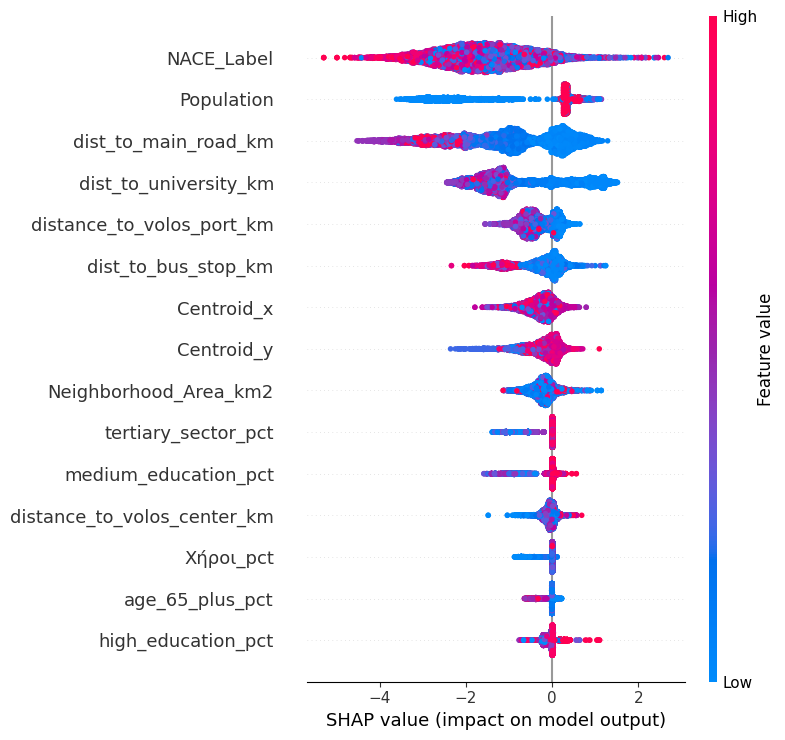
\includegraphics[scale=0.4]{figures/shap_average.png}
    \centering
    \caption{Average SHAP Values of all Features}
    \label{fig:shap_average}
\end{figure}


%==================================================
\subsubsection{Feature Statistics \& Feature Justification}
\label{sec:feature_justification}

The SHAP values displayed in the previous section described which features will be jutified, but did not explain how. To provide informative justifications for each feature, I calculated specific statistics per feature, namely the 25th, 50th, and 75th percentiles (q25, q50, q75). During feature justification, each feature value is compared with these percentiles to determine its corresponding interval. For every interval, 3 justification templates have been generated by ChatGPT, one of which is randomly selected to provide variation. From this point forward, we will refer to this process as "feature justification". Figure \ref{fig:feature_justification} visually demonstrates the different templates used based on the value and statistics.

\begin{figure}[!htbp]
    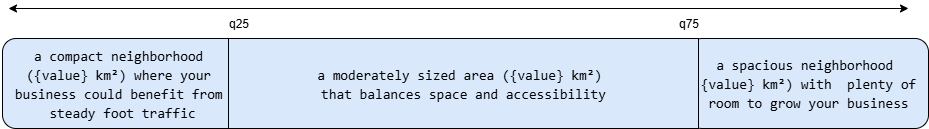
\includegraphics[scale=0.4]{figures/feature_justification.png}
    \centering
    \caption{Feature Justification for 'Neighborhood\_Area\_km2'}
    \label{fig:feature_justification}
\end{figure}


%==================================================
\subsubsection{Neighborhood Justification}
\label{sec:neigh_justification}

During the construction of training completions, we aim to provide explainable outputs which justify each recommendation. Building on the feature justification method described above, a complete reasoning about a neighborhood can be implemented by aggregating the justifications of several features. At this stage, it becomes essential to select certain features, as using them all would result in an overly large output. 

Six features were used to provide explainability to the output. Certain features, assumed to be consistently important, were treated as "fixed". Examples include neighborhood area, proximity to the city center, and distance from highways \ref{tab:fixed_features}. During neighborhood justification, 4 out of 7 fixed features are randomly selected and justified. The two remaining features were selected according to their SHAP values, specifically choosing the two most important features not included among the fixed ones. This combination of fixed features with SHAP importance balances consistency with variety of the training output.


%==================================================
\subsubsection{Prompt Construction}

The creation of training prompts is relatively straightforward. They are based on five synthetic templates generated by ChatGPT, each parametrised by the business category. When constructing the fine-tuning dataset the synthetic category is passed as input. Table \ref{tab:prompt_templates} displays the synthetic prompt templates. We generate one template per synthetic category, resulting in a total amount of 918.


\begin{table}[ht!]
    \centering
    \begin{tabular}{|M{10cm}|}
        \hline
        \textbf{Prompt Templates} \\ \hline
        "Where should I open a \textbf{\{category\}} in Volos?" \\ \hline
        "What is the best neighborhood in Volos for a \textbf{\{category\}}?" \\ \hline
        "I'm looking to start a \textbf{\{category\}}. Which area would be ideal in Volos?" \\ \hline
        "Suggest a location in Volos for a \textbf{\{category\}}." \\ \hline
        "Which place would you recommend for opening a \textbf{\{category\}} business in Volos?" \\ \hline
    \end{tabular}
    \caption{Synthetic Prompt Templates}
    \label{tab:prompt_templates}
\end{table}


%==================================================
\subsubsection{Completion Construction}
\label{sec:completion_construction}

The construction of training completions involves the justification mechanisms mentioned above. For every synthetic category, we extract the proxy top 3 recommendations of its corresponding NACE class as estimated in section \ref{sec:proxy}. The recommendations are transformed to explanatory text by applying the neighborhood justification method described previously \ref{sec:neigh_justification}, and combined to form the final completion. The workflow is shown intuitively in Figure \ref{fig:completion}.

\begin{figure}[h]
    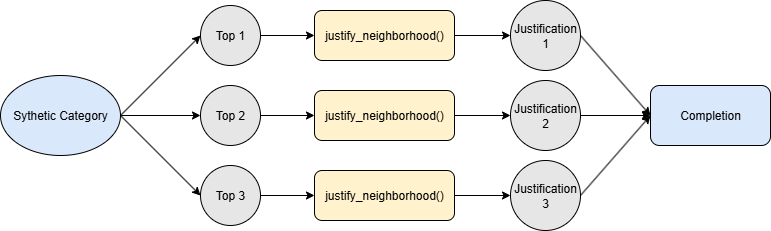
\includegraphics[scale=0.5]{figures/completion.png}
    \centering
    \caption{Completion Construction Workflow}
    \label{fig:completion}
\end{figure}


%==================================================
\subsubsection{Prompt-Completion Example}

To illustrate the fine-tuning dataset creation process, we present a prompt-completion pair generated for the synthetic category "greenhouse farming" that corresponds to the NACE class 1.13 in \ref{ex:prompt_completion_greenhouse}. The total prompt-completion pairs are 918 as mentioned before.

\begin{figure}[htbp]
  \centering
  \begin{tcolorbox}[myexample, title={Prompt-Completion Example}]
  \textbf{Prompt:} \emph{Where should I open a greenhouse farming business in Volos?}

  \vspace{0.5\baselineskip}
  \textbf{Completion:} \emph{Top neighborhoods for a Greenhouse farming business (NACE 1.13: Growing of vegetables and melons, roots and tubers) in Volos:}
  \begin{enumerate}
    \item \textbf{Metamorfosi} -- right near the university (0.14 km) --- great if you want to attract students or young professionals; a large local population, which can bring in steady foot traffic; a compact neighborhood (0.56 km$^{2}$) where your business could benefit from steady foot traffic; excellent central location (0.54 km), making your business easy to find and reach; accessible without being too exposed to street noise or congestion (0.16 km); fairly accessible by public transport (0.20 km), even if not right next to a bus stop.
    \item \textbf{Kato Lehonia} -- a balanced location (2.07 km$^{2}$) --- not too dense, not too open; a busy neighborhood with a strong base of potential customers nearby; close enough (8.62 km) to be convenient, while still offering some breathing room from downtown traffic; great access to main roads (0.01 km) --- easy for customers to reach you and for deliveries to run smoothly; not close to campus (8.21 km), which could work well for businesses focused on the neighborhood itself; excellent access to public transit (0.04 km), which can boost foot traffic to your business.
    \item \textbf{Agios Konstantinos} -- a moderately sized area (0.82 km$^{2}$) that balances space and accessibility; it's very close to the city center (1.41 km), which means great visibility and easy access; a reasonable distance from transit (0.16 km) --- close enough for most customers to reach you without much hassle; lots of people live in the area --- great for attracting walk-in customers; reasonably close to main roads (0.13 km), giving you decent accessibility without heavy traffic; a lively spot near the university (0.82 km) that could bring in a lot of student activity.
  \end{enumerate}
  \end{tcolorbox}
  \caption{Prompt-Completion Example}
  \label{ex:prompt_completion_greenhouse}
\end{figure}



%==================================================
%==================================================
\subsection{Inference Dataset Creation}
\label{sec:inference_dataset}

The construction of the inference dataset is similar to that of the training dataset, differing only in the synthetic categories used. Αll NACE classes were divided into two categories based on their frequency on the business entries dataset: classes that characterize at least 50 businesses were considered main classes, otherwise they are treated as secondary. The main classes are 53 and comprise almost 63.32\% of the total businesses. During the inference data creation only main classes are used. This is done to provide a more realistic model evaluation, as keeping only frequent business types results in an inference dataset representative of real-world examples. As before, 3 synthetic categories per class were generated, accounting for 3x53 = 159 total entries. The construction of the prompts and completions is identical to that described previously.


%==================================================
%==================================================
\subsection{Fine-Tuning Process}

After showing the construction of the training dataset, we can finally examine the fine-tuning process. Below, we mention details like computational recourses, the base model, and the fine-tuning techniques applied.


%==================================================
\subsubsection{Hardware \& Base Model}

The training was carried out on the high-performance computing cluster of University of Thessally, that utilizes an NVIDIA A100 GPU. Given our hardware capabilities, "mistralai/Mistral-7B-Instruct-v0.2" was chosen for its balance between strong instruction-following capabilities and computational efficiency. 

%==================================================
\subsubsection{Quantization \& QLoRA}

Fine-tuning was preformed using the QLoRA (Quantized Low-Rank Adaption) method, which combines quantization of the base model with integration of lightweight trainable adepter layers. In order to fit the 7 billion parameter within the available GPU memory, the base model weights were loaded in 4-bit NF4 quantization and kept frozen during training. Since these weights remain unchanged, LoRA adapters, specificlly 16-rank matrices, were inserted as trainable parameters. When the parameters of the model are printed, we get the values shown on Table \ref{tab:qlora}. The total parameters are displayed to be around 3.75 instead of 7 billion due to the compressed representation after quantization. In addition, the tiny percentage of trainable parameters demonstrates the effect of QLoRA adapters, resulting in a significantly more lightweight model with only 0.1813\% trainable weights.\\

\begin{table}[ht!]
    \centering
    \begin{tabular}{|p{5cm}|p{5cm}|}
        \hline
        Total Parameters & 3.758.895.104 \\
        \hline
        Trainable parameters & 6.815.744 \\ \hline
        Trainable \% & 0.1813\% \\ \hline
    \end{tabular}
    \caption{Model Parameters after QLoRA}
    \label{tab:qlora}
\end{table}


%==================================================
\subsubsection{Tokenization \& Label Masking}

Before performing the model fine-tuning, each prompt-completion example was converted to compatible formatting for the Mistral-Instruct tokenizer, using the template \ref{eq:inst_format}. The formatted string is then tokenized using a fixed length, either by truncation or padding, set to 512 after determining that 95\% of the formatted strings result in 462 or less tokens.

\begin{equation}
    \texttt{<s>[INST] {prompt} [/INST] {completion} </s>}
    \label{eq:inst_format}
\end{equation}

To ensure the model learns to predict only the completion and not the prompt, the labels of the instruction's tokens are masked out by setting their value to -100 so they get ignored when computing the crossentropy loss function.

%==================================================
\subsubsection{Training Configuration}

As we previously mentioned, 4-bit NF4 quantization was used along with QLoRA adapters of rank 16. The scaling factor, which determines the influence of the adapters, is set to 64, which is a balanced, standard choice. During the training we used an effective batch size per device of 2 and a gradient accumulation of 4, resulting in a total effective batch size of 8. The learning rate was set to 2e-5. The complete training configurating is displayed on table \ref{tab:finetune_config}. Regarding the number of epochs, three attempts were made with 3, 5, and 8 epochs respectively. The results will be further explored in chapter 5.


%==================================================
%==================================================
\subsection{Fine-Tuned LLM Workflow Summary}


So far we described the complete fine-tuning process. After training the model, its workflow is relatively straight forward. The LLM is simply fed a text input, and produces the predicted output. We showcase the workflow here to compare it later with the RAG pipeline, whose workflow is a bit more complex. Figure \ref{fig:workflow_ft} provides an intuitive visualization of the system.

\begin{figure}[h]
    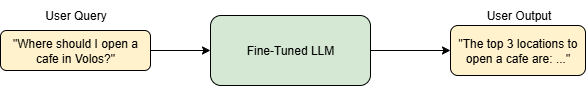
\includegraphics[scale=0.5]{figures/workflow_ft.png}
    \centering
    \caption{Fine-Tuned LLM Workflow}
    \label{fig:workflow_ft}
\end{figure}



%==================================================
%==================================================
\subsection{Inference Process}

After performing model fine-tuning, the resulting LLM is used on the inference dataset described in \ref{sec:inference_dataset}. This process was also run on the NVIDIA A100 GPU of University of Thessally. To ensure computational efficiency, inference was performed in batches of size 8. The outputs are stored, as they will be used later to evaluate the model performance by comparing them to the completions created in section \ref{sec:completion_construction}.




%==================================================
%==================================================
%==================================================
\section{RAG with Re-Ranking Pipeline}
\label{sec:rag}

This section explores the second state-of-the-art method that was implemented, a Retrieval-Augmented Generation workflow. First, we examine the motivation for exploring this method despite having already implemented the LLM fine-tuning approach. Followingly, we will show the creation of neighborhood descriptions that will be utilized in the framework. Finally, we will present the complete RAG pipeline, including the selected embedder, its application, and the integration with a generative LLM to produce the final output.



%==================================================
%==================================================
\subsection{Motivation}

While fine-tuning an LLM as described in section \ref{sec:fine_tuned_llm} indeed utilizes generative AI in an innovative way to address the problem of business location recommendation, it presents several important constraints. Adding proxy truths for new NACE classes or modifying existing ones requires re-running the entire fine-tuning process, which is both time consuming and computationally expensive. The desire to avoid this makes the approach static. Moreover, the justifications may not always include valid numbers, since LLMs are prone to hallucinations. Furthermore, since the model essentially learns to predict three static recommendations per NACE class, personalization may be difficult if users have specific preferences. A Retrieval-
Augmented Generation can potentially handle these problems because its memory is not stored inside the LLM and can be updated without extensive training In addition, the system outside of the LLM can adjust the final recommendations based on specific user desires, potentially allowing for better personalization.



%==================================================
%==================================================
\subsection{Neighborhood Description Creation}
\label{sec:neigh_desc}

Looking forward, we aim to compare the initial user query with the candidate locations to recommend the appropriate ones. Since the query is a text input which can be embedded into a dense vector representation, the first step was to create a text description per neighborhood that will later be also embedded and compared with the user query. The creation of descriptions is based on the core concepts used in the fine-tuning dataset construction \ref{sec:fine_tune_dataset_creation}, specifically the neighborhood justification method which essentially integrates multiple feature justifications.


%==================================================
\subsubsection{Feature Statistics \& Feature Justification}

This process is identical to the feature justification workflow explained in section \ref{sec:feature_justification}. The same statistic values are calculated for every feature, resulting in a specific text justification depending on the comparison of the individual feature's value in comparison with its percentiles. Once more, we randomly select one out of three templates per precentile interval for variety.


%==================================================

\begin{figure}[htbp]
  \centering
  \begin{tcolorbox}[myexample, title={Neighborhood Description}]
  \vspace{0.5\baselineskip}
  \textbf{Agios Nikolaos:} \emph{Neighborhood description:\\}
    A cozy location (0.35 km$^{2}$) that might work well for storefronts or quick-service ideas; it's very close to the city center (0.90 km), which means great visibility and easy access; very close to the port (0.53 km), which makes transport and logistics a lot easier; great access to main roads (0.00 km) — easy for customers to reach you and for deliveries to run smoothly; excellent access to public transit (0.01 km), which can boost foot traffic to your business; close to campus (0.09 km), which means steady foot traffic from a younger, educated crowd; a busy neighborhood with a strong base of potential customers nearby; a neighborhood with many single adults (40\%) — ideal for modern, fast-moving business models; fewer married residents (46\%), which could favor services tailored to individuals or younger adults; not a heavily elderly area (8\%), which could favor modern, fast-paced, or tech-forward businesses.
  \end{tcolorbox}
  \caption{Description for Agios Nikolaos}
  \label{fig:description_agiosnikolaos}
\end{figure}

\subsubsection{Neighborhood Description}
\label{sec:neigh_description}

The generation of descriptions is very similar to the construction of neighborhood justifications described previously \ref{sec:neigh_justification}, with some minor modifications. The major difference is that, in this case, producing large text is not a problem. While previously these justifications were used as LLM outputs and therefore had to be constrained, in this case, we aim to embed them. Hence, including as much information as possible about the neighborhood is not only acceptable but beneficial.

In more detail, the same fixed features are used \ref{tab:fixed_features}, but a justification is provided for all of them rather than only a subset. The total number of features used is also increased, resulting in a larger amount of secondary features as well. In \ref{fig:description_agiosnikolaos} we provide an indicative example of a neighborhood description.




%==================================================
%==================================================
\subsection{Embedding and Retrieval Process}

The RAG pipeline uses an embedder model that transforms text descriptions into high-dimensional dense vector representations. This enables similarity search between user queries and neighborhood descriptions. 



%==================================================
\subsubsection{Embedder Model}

To perform the embeddings, we selected the model "BAAI/bge-large-en-v1.5". This is a BERT-style transformer encoder with about 335 million parameters, optimized for semantic similarity search and RAG pipelines. It uses a vocabulary size of 30.522 tokens, 24 transformer layers, and the generated embeddings are of dimension 1024.


%==================================================
\subsubsection{Embedding NACE Descriptions}
\label{sec:embedding_nace}

As we will explain later, after acquiring the user query, the first step is to determine the NACE class of the business the user wants to open. This will be done by performing a vector similarity search between the query embedding and all NACE class descriptions. To avoid embedding all NACE descriptions in real time, we precompute the vector representations once and store them, allowing them to be retrieved during runtime. They are stored in the JSON file 'nace\_descriptions\_embeddings.json'.


%==================================================
\subsubsection{Embedding Neighborhood Descriptions}
\label{sec:embedding_neigh}

After determining the NACE code, we could simply use its corresponding proxy truths to provide the recommendations. In order to allow better personalization, however, we utilize a re-ranking method that initially fetches the top 10 suggestions, and re-ranks them based on vector similarity between them and the user query. This requires embedding the neighborhood descriptions created in section \ref{sec:neigh_description}. As we previously did with the NACE descriptions, the embedding generation of neighborhood descriptions is performed once, and stored in the JSON file 'neighborhoods\_descriptions\_embeddings.json'.


%==================================================


\subsubsection{Retrieval Process Output}

The re-ranking process results in an updated sorted list of top 10 recommendations. Since the structure of the final output should consist of three suggestions, we simply select the three most similar neighborhoods. Figure \ref{fig:retrieval} demonstrates the complete retrieval process as described in the previous sections.



\begin{figure}[!htbp]
    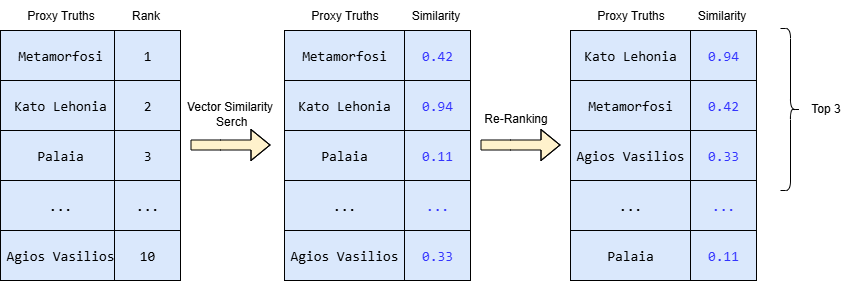
\includegraphics[scale=0.5]{figures/retrieval.png}
    \centering
    \caption{Retrieval Process}
    \label{fig:retrieval}
\end{figure}


%==================================================
%==================================================
\subsection{LLM Integration}

The retrieval process extracts the final suggestions that are intended to be presented to the user. In order to present them in a coherent, user-friendly recommendation, we utilize an LLM that receives the raw recommendations and descriptions and produces the final output message. In contrast with the fine-tuned LLM approach, in this case the LLM does not decide the actual recommendations, it acts only as the output generator.



%==================================================
\subsubsection{Selected LLM}

For user output generation, Llama 3 (8 billion parameters) was used. The model is run locally via Ollama, and thus is loaded in 4-bit quantization to ensure compatibility with the local hardware. It supports a context length of 8192 tokens and embedding dimensionality of 4096. During retrieval-augmented generation, the model is simply fed a specifically structured input and inferred to obtain the user output.


%==================================================
\subsubsection{LLM Prompt Construction \& Final Output}

To ensure clarity and user-friendly outputs, a structured template was constructed to guide the final output of the LLM. The template initially specifies the user query with the extracted NACE class and its description. Next, it mentions the three recommendations with their descriptions, and finishes by providing certain explicit output instructions. Figure \ref{fig:llm_prompt} shows an indicative example of the LLM prompt constructed to provide recommendations to the query "Where in Volos should I start a bakery business?". The descriptions are incomplete to fit the whole prompt. After the LLM prompt is constructed, we simply feed it to the model and infer it to acquire the final output. This is the final response that the user receives from our system.
 

\begin{figure}[!htbp]
  \centering
  \begin{tcolorbox}[myexample, title={LLM Prompt Example}]
  \vspace{0.5\baselineskip}
    The user wants to open a business of type: "Where in Volos should I start a bakery business?"\\
    **NACE Code: 46.36 — Wholesale of sugar and chocolate and sugar confectionery**\\
    Based on data analysis, here are the top 3 recommended neighborhoods in Volos:\\
    
    **Hiliadou** – a balanced location (1.03 km²) — not too dense, not too open, you'll be right near the heart of Volos (1.17 km) — convenient for both customers and deliveries, ...\\
    
    **Karagats** – a cozy location (0.67 km²) that might work well for storefronts or quick-service ideas, it's very close to the city center (0.98 km), which means great visibility and easy access, ...\\
    
    **Metamorfosi** – a cozy location (0.56 km²) that might work well for storefronts or quick-service ideas, you'll be right near the heart of Volos (0.54 km) — convenient for both customers and deliveries, ...\\
    
    Please present the 3 neighborhoods in a numbered list format like this:\\
    1. Neighborhood Name: Summary of strengths...\\
    2. Neighborhood Name: Summary of strengths...\\
    3. Neighborhood Name: Summary of strengths...\\
    Each point should be 2–4 sentences long, clearly explaining why the neighborhood is a good fit for the business. Avoid ranking or comparisons — describe each one positively and independently.
  \end{tcolorbox}
  \caption{LLM Prompt Example}
  \label{fig:llm_prompt}
\end{figure}



%==================================================
%==================================================
\subsection{RAG Pipeline Workflow Summary}

In the previous sections we examined the individual parts of the RAG framework. Here, we present a summary of the complete workflow. The system first receives the user query that asks about a specific type of business. Using the embedder, the entry is converted into a high-dimensional vector in real time. We find the corresponding NACE class of the business type by calculating the similarity between the query embedding, and the embedding of all NACE descriptions, which are pre-computed and stored locally. Next, we fetch the top 10 proxy recommendations of the NACE class, and apply vector semantic similarity once more, this time between the query and the neighborhood embeddings which are also available locally. The similarities are used as the re-ranking criterion to acquire personalized suggestions.   

The three neighborhoods with higher similarity scores are the final recommendations. In order to return a cohesive and context-aware message to the user, we pass the recommendations and their descriptions to a specifically structured template, and feed this to the Llamma 3 LLM to produce the final output. Figure \ref{fig:rag_workflow} visually shows the complete pipeline.


\begin{figure}[h]
    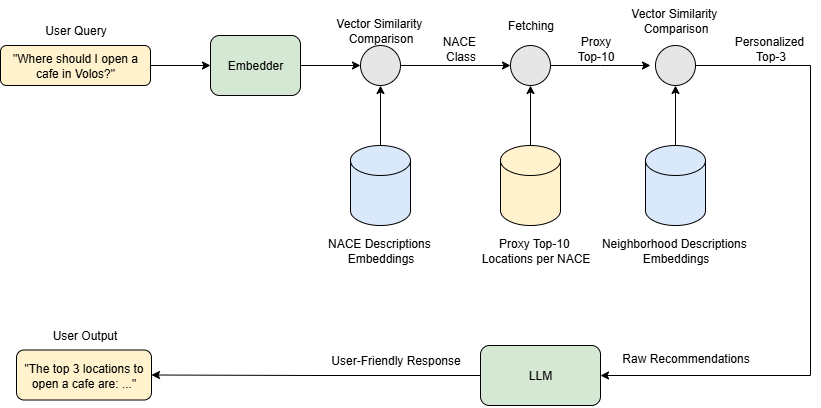
\includegraphics[scale=0.5]{figures/rag_workflow.png}
    \centering
    \caption{RAG Pipeline}
    \label{fig:rag_workflow}
\end{figure}


%==================================================
%==================================================
\subsection{Inference Process}
\label{sec:inf_rag}

After implemention the complete RAG pipeline, it is used on the inference dataset described in \ref{sec:inference_dataset}. In contrast to the fine-tuned LLM inference, this process is run locally since the loaded embedder is of reasonable size (355 million parameters) and the loaded LLM is quantized. The outputs are stored, as they will be used later to evaluate the pipeline performance by comparing them to the completions created in section \ref{sec:completion_construction}.



%==================================================
%==================================================
%==================================================
\section{Chatbot Interface}

The previous sections \ref{sec:fine_tuned_llm} and \ref{sec:rag} essentially describe the process of constructing frameworks that receive a text input and return a text output. In order to create a user-friendly application we create a chatbot-like interface. This section describes the frontend and backend development of the application, highlighting the mechanism that transforms simple LLMs into chatbots by memorizing the conversation.

%==================================================
%==================================================
\subsection{Frontend Development}

The frontend construction regards the form of the final user interface. Below we describe details of the fontend implementation. We start by mentioning why we chose the 'Streamlit' library, then showcase the interface design, and finally explain how the chat memory is stored in the frontend.


%==================================================
\subsubsection{Streamlit Framework}

Streamlit is an open-source Python framework designed to develop application frontends in a simple and efficient manner. Unlike traditional web frameworks, like React or Django, which require extensive knowledge of front-end technologies, Streamlit supports direct implementation in Pythn scripts. This makes it a great option for deploying machine learning models, where our primary goal is to provide a simple user interface rather than create a complex application. In the context of this thesis, Streamlit was utilized to implement the chatbot interface, as it provides a built-in session management and a simple layout system that can be easily integrated with a Python backend. \\



%==================================================
\begin{figure}[h]
    \centering
    \fbox{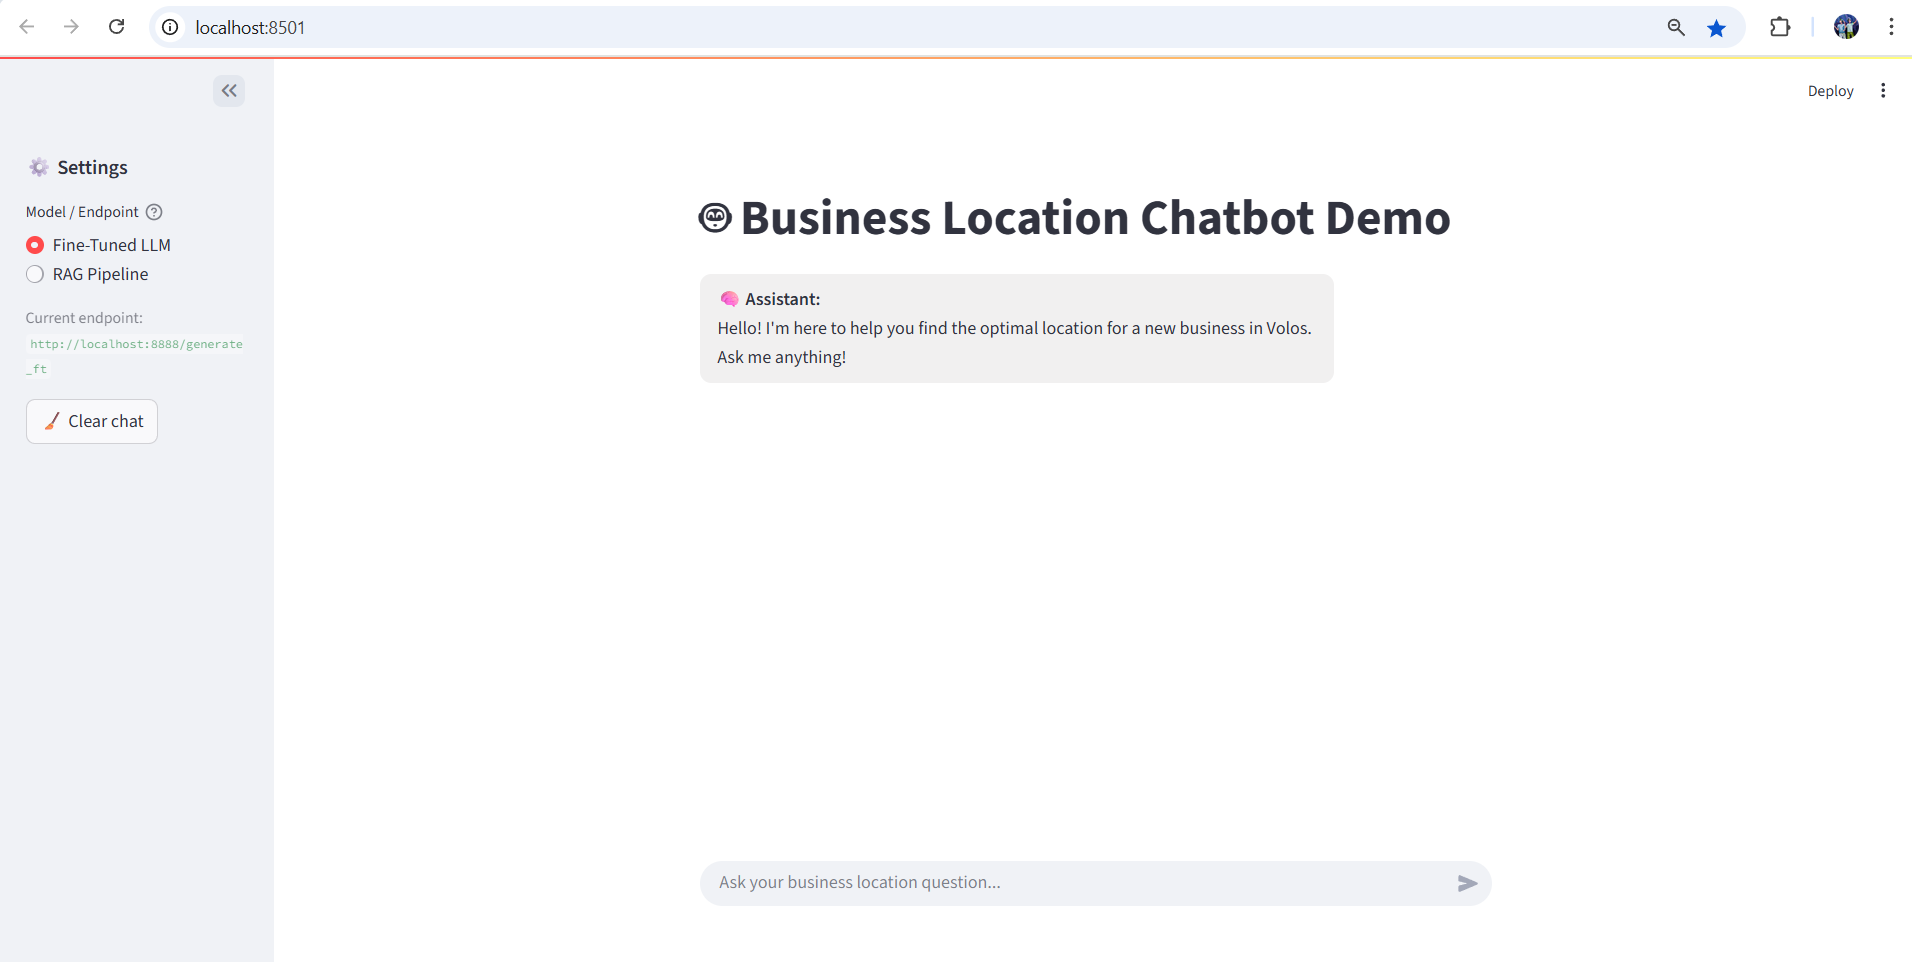
\includegraphics[scale=0.35]{figures/interface.png}}
    \caption{User Interface Design}
    \label{fig:interface}
\end{figure}


\subsubsection{User Interface Design}

The application design aims to mirror a state-of-the-art interface that provides a user-friendly experience. The page is initialized with the title "Business Location Chatbot Demo" and a greeting message from the AI assistant. At the bottom of the screen, an input box expects the input of the user. To improve readability, the conversation messages were designed with simple HTML and CSS embedded in Streamlit \ref{lst:render_user}, \ref{lst:render_assistant}. The assistant messages are shown in gray and aligned to the left, with the title "Assistant:". In contrast, the user messages appear in blue color, aligned to the right, and using the title  "You:". The interface dynamically updates after every new message. To ensure a continuous flow of conversation, when a user query is submitted, a spinner animation is displayed until the request is completed, and the response is displayed as well. The interface also contains a sidebar, that allows the user to select the backend system used, which we further explain in section \ref{sec:backend_development}. Figure \ref{fig:interface} shows an indicative screenshot of the application design, along with the greeting message.


%==================================================
\subsubsection{Session \& Memory Management}

During Streamlit sessions, the Python script is re-executed on every user interaction. In order to save the conversation history, we use the 'st.session\_state' object, which contains messages within the same session. The messages are stored as JSON objects, with fields: 'role', which identifies wether this is a user or assistant message, and 'content', which contains the actual message. At the beginning of a new session, the session state is initialized only with the greeting message. Every new message, whether from the user or the assistant, is integrated into the state. This mechanism essentially stores the conversation memory in the frontend. The complete history is then forwarded to the backend and processed from there, as we will analyze below.



%==================================================
%==================================================
\subsection{Backend Development}
\label{sec:backend_development}

The backend acts as the bridge between the user interface and the AI models. It is responsible for handling requests from the frontend, producing the output by using the systems we implemented, and returning it as a response. Below, we explain the framework selected to build the backend and the endpoint functions for each method. It is important to highlight that, while the inference of the RAG framework ran locally \ref{sec:inf_rag}, in order to use one server for the application, we run both approaches remotely on the computational cluster of University of Thessally.


%==================================================
\subsubsection{FastAPI Framework}

FastAPI is a modern Python framework, specifically designed for building APIs efficiently. Compared to traditional frameworks such as Flask or Django, FastAPI is lightweight and more simple. One of its main advantages is the support of asynchronous requests, which makes it suitable for long-running processes. This makes it ideal for our case, as querying a language model can be modeled in this framework.



%==================================================
\subsubsection{Fine-Tuned LLM Pipeline}
\label{sec:backend_ft}

The fine-tuned LLM approach is wrapped in the FastAPI endpoint '/generate'. When the Python script starts running, we load the LLM ('mistralai/Mistral-7B-Instruct-v0.2') in 4-bit quantization and attach the LoRA adapters created during fine-tuning on top of it. Once the model is active, it listens for user queries. The process is almost identical to the simple inference of the fine-tuned LLM system, with minor changes. In order to transform a simple LLM module into a chatbot, we simply have to modify the system input. 

\begin{figure}[h]
    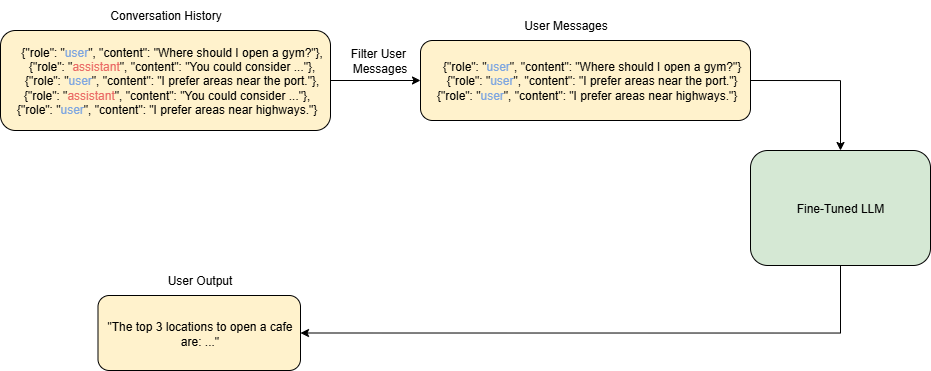
\includegraphics[scale=0.35]{figures/backend_ft.png}
    \centering
    \caption{Backend Fine-Tuned LLM Pipeline}
    \label{fig:backend_ft}
\end{figure}

As described previously, when a user query is received, a request is made from the frontend to the backend, containing the complete conversation history. The fine-tuned LLM extracts only the user messages and concatenates them to create the complete input. We treat the first user message as the ’intent’, since we assume that it contains the desired business type. The rest of them are treated as ’constraints’, based on the assumption that the follow-up messages specify preferences of the user. By combining the intent and constraints we create a prompt that always contains the desired NACE class, and also is up to date with every user specification. Figure \ref{fig:backend_ft} demonstrates this workflow.



%==================================================
\subsubsection{Retrieval-Augmented Generation Pipeline}
\label{sec:backend_rag}

The Retrieval-Augmented Generation pipeline is wrapped in the FastAPI endpoint '/generate\_rag'. In the beginning of the Python script, we load the embedder model ('BAAI/bge-large-en-v1.5') with its tokenizer, and we fetch the pre-computed embeddings of the NACE and neighborhoods descriptions described in section \ref{sec:embedding_nace}. The process again mirrors the inference of the system.

\begin{figure}[h]
    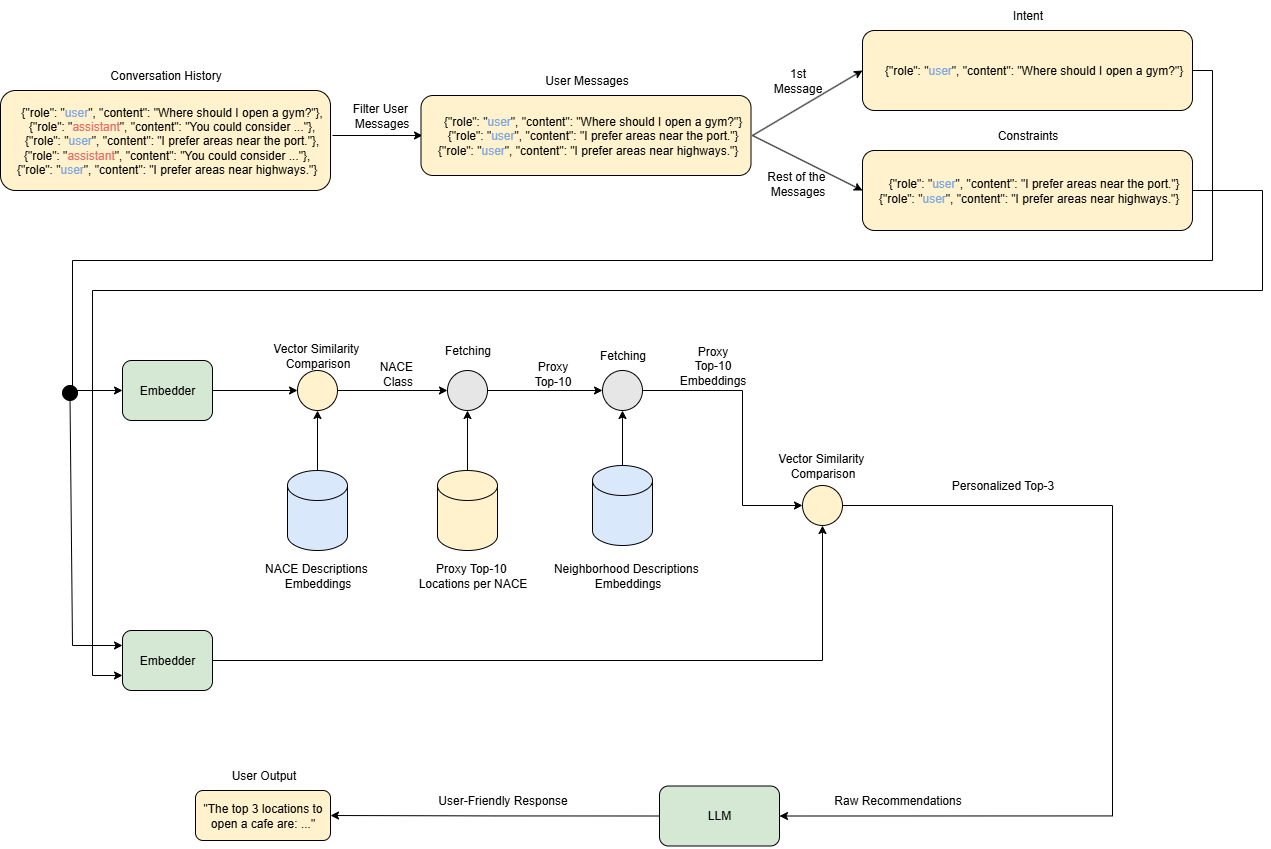
\includegraphics[scale=0.35]{figures/backend_rag.png}
    \centering
    \caption{Backend RAG Pipeline}
    \label{fig:backend_rag}
\end{figure}

The RAG system also extracts only user messages. We use just the intent to specify the NACE class, as the constraints should not affect the type of the business, only the actual recommendations. During the re-ranking, we embed the intent along with the constraints to fetch the final suggestions. Figure \ref{fig:backend_rag} shows the workflow visually.




%==================================================
%==================================================
\subsection{Frontend-Backend Communication}

The frontend communicates with the backend using synchronous HTTP POST requests to FastAPI endpoints. FastAPI provides a lightweight and JSON-friendly communication protocol that can easily be integrated with the Streamlit interface. Two main endpoints are available: '/generate', for deploying the fine-tuned LLM approach described in section \ref{sec:backend_ft}, and '/generate\_rag' for the RAG system pipeline explained in section \ref{sec:backend_rag}. The request messages send a JSON payload that contains the complete conversation history, together with a fixed system prompt that guides the output of the selected system \ref{fig:system_prompt}.\\


\begin{center}
    \fbox{\parbox{0.8\linewidth}{
    \textit{"You are a helpful assistant that suggests optimal business locations in Greece based on demographics and area characteristics."}
    }}
    \captionof{figure}{System Prompt for LLM Guidance}
    \label{fig:system_prompt}
\end{center}

The complete communication process can be summarized as follows: The frontend receives the user input, integrates it to the conversation, forwards the updated conversation history to the backend, which processes it, generates a response, and returns it. This approach ensures a clear and modular role for each side of the system. Figure \ref{fig:communication} intuitively displays the communication workflow between the frontend and the backend.\\

\begin{figure}[h]
    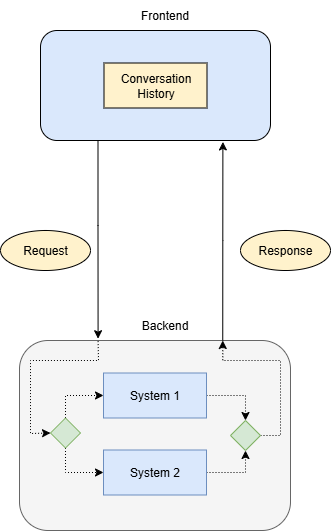
\includegraphics[scale=0.35]{figures/communication.png}
    \centering
    \caption{Frontent-Backend Communication}
    \label{fig:communication}
\end{figure}



%==================================================
%==================================================
\subsection{Chatbot Demo}

The previous sections described the process of transforming an LLM-based system, which simply receives a text input to a text output, to a chatbot application, with memory for the conversation history and a complete fontend-backend communication system. Below, we present an example of a conversation for every approach to demonstrate the results.


%==================================================
\subsubsection{Fine-Tuned LLM Approach}

Figure \ref{fig:chatbot_inf_ft} shows an example of a conversation using the fine-tuned LLM. We see that the structure of the output resembles the training data, which is expected, since the LLM learns to follow this specific pattern. In this case, we see a mistaken prediction, since the constraint about areas close to the ports actually results in a number 1 option, whose port distance is larger than options 2 and 3.

\begin{figure}[h!]
    \centering
    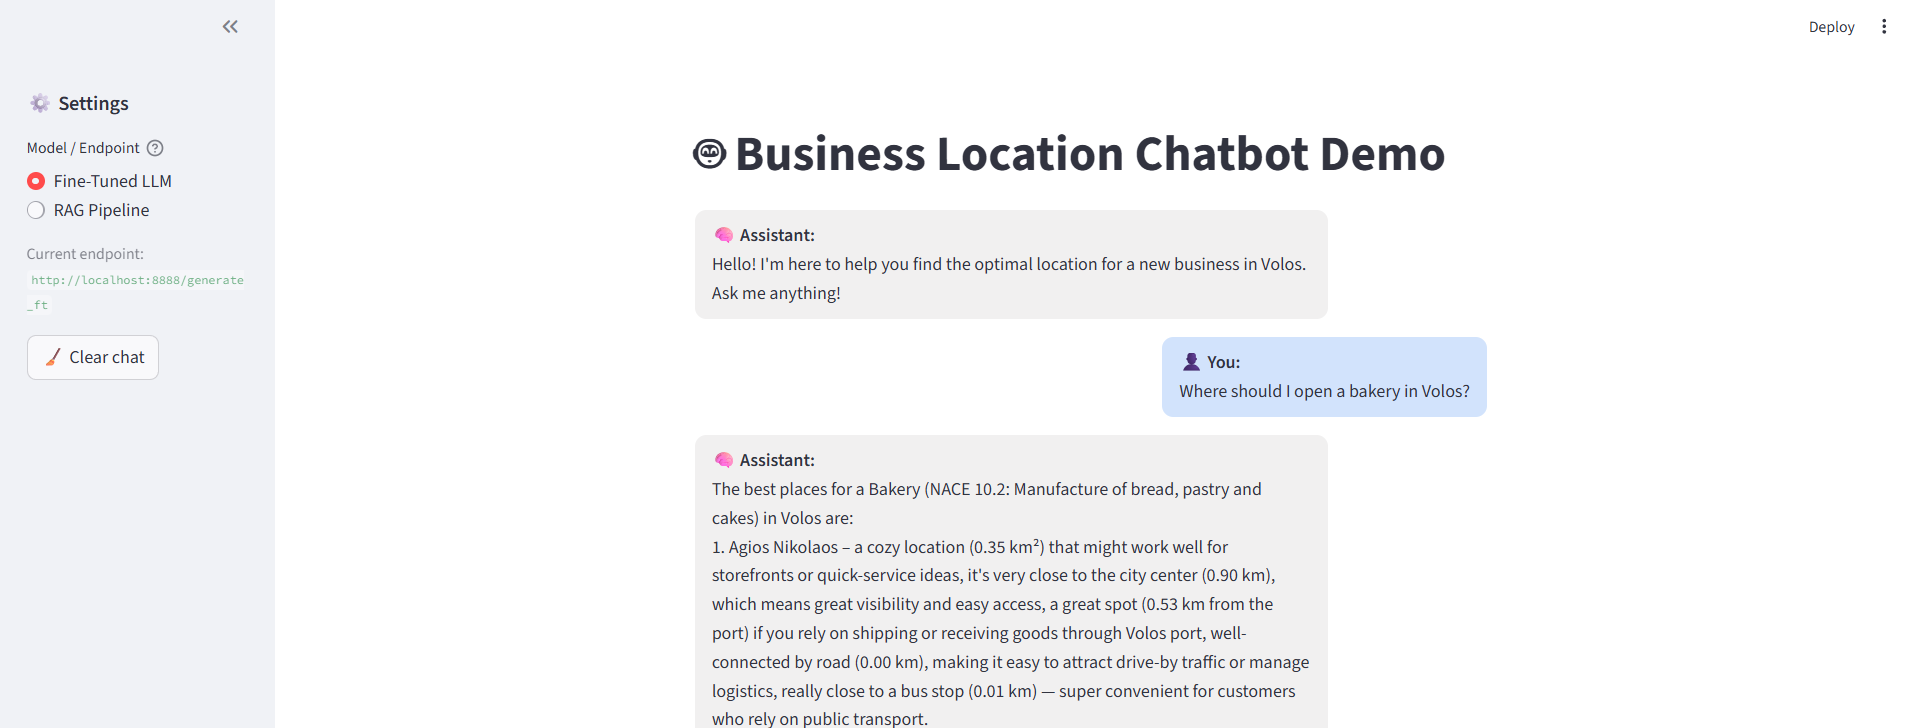
\includegraphics[width=0.8\textwidth]{figures/inf_chatbot_ft_1.png}\\[0.5em]
    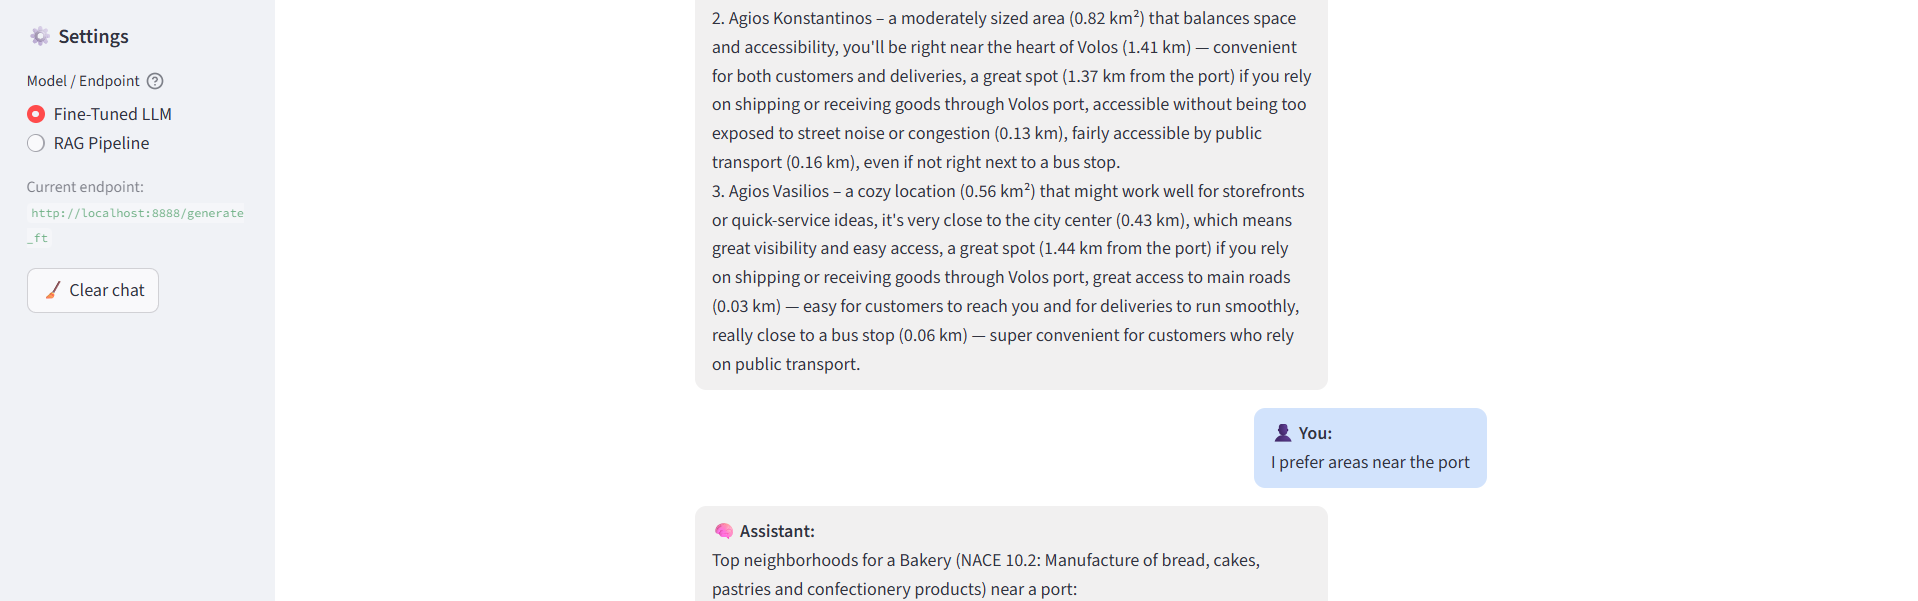
\includegraphics[width=0.8\textwidth]{figures/inf_chatbot_ft_2.png}
    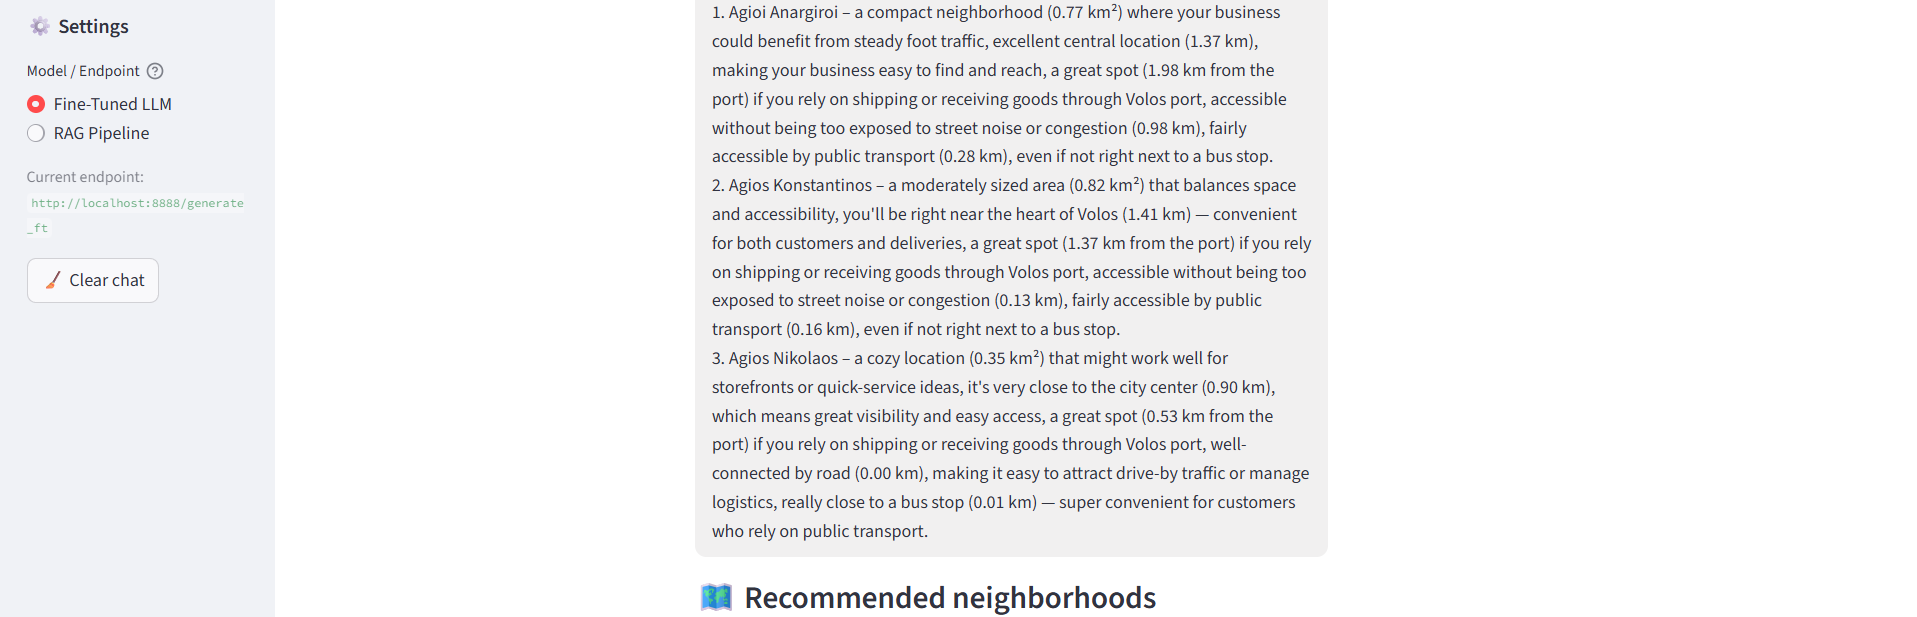
\includegraphics[width=0.8\textwidth]{figures/inf_chatbot_ft_3.png}
    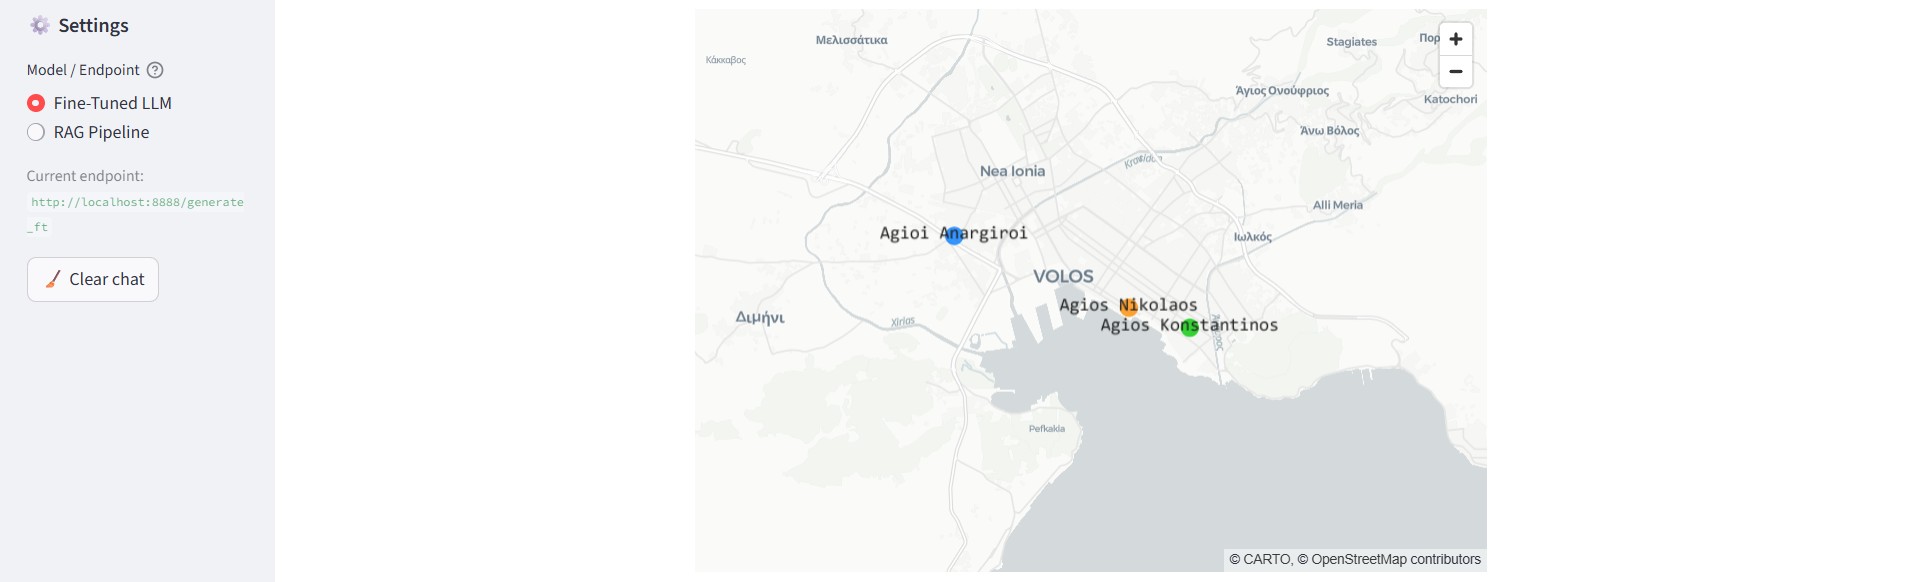
\includegraphics[width=0.8\textwidth]{figures/inf_chatbot_ft_4.png}
    
\includegraphics[width=0.8\textwidth]{figures/inf_chatbot_ft_5.png}
    \caption{Chatbot Inference - Fine-Tuned LLM Approach}
    \label{fig:chatbot_inf_ft}
\end{figure}



%==================================================
\subsubsection{RAG Pipeline Approach}

Figure \ref{fig:chatbot_inf_rag} shows an instance of  the conversation that occurs by the RAG pipeline. In contrast with the fine-tuned LLM, this output follows a slightly different reasoning format because the generator is not trained on following the structure of the training data. This time the chatbot actually changes its prediction in the correct direction, as the port distance constraint produces Palaia as the first recommendation, which is closer to the port than the old recommendation. 


\begin{figure}[h!]
    \centering
    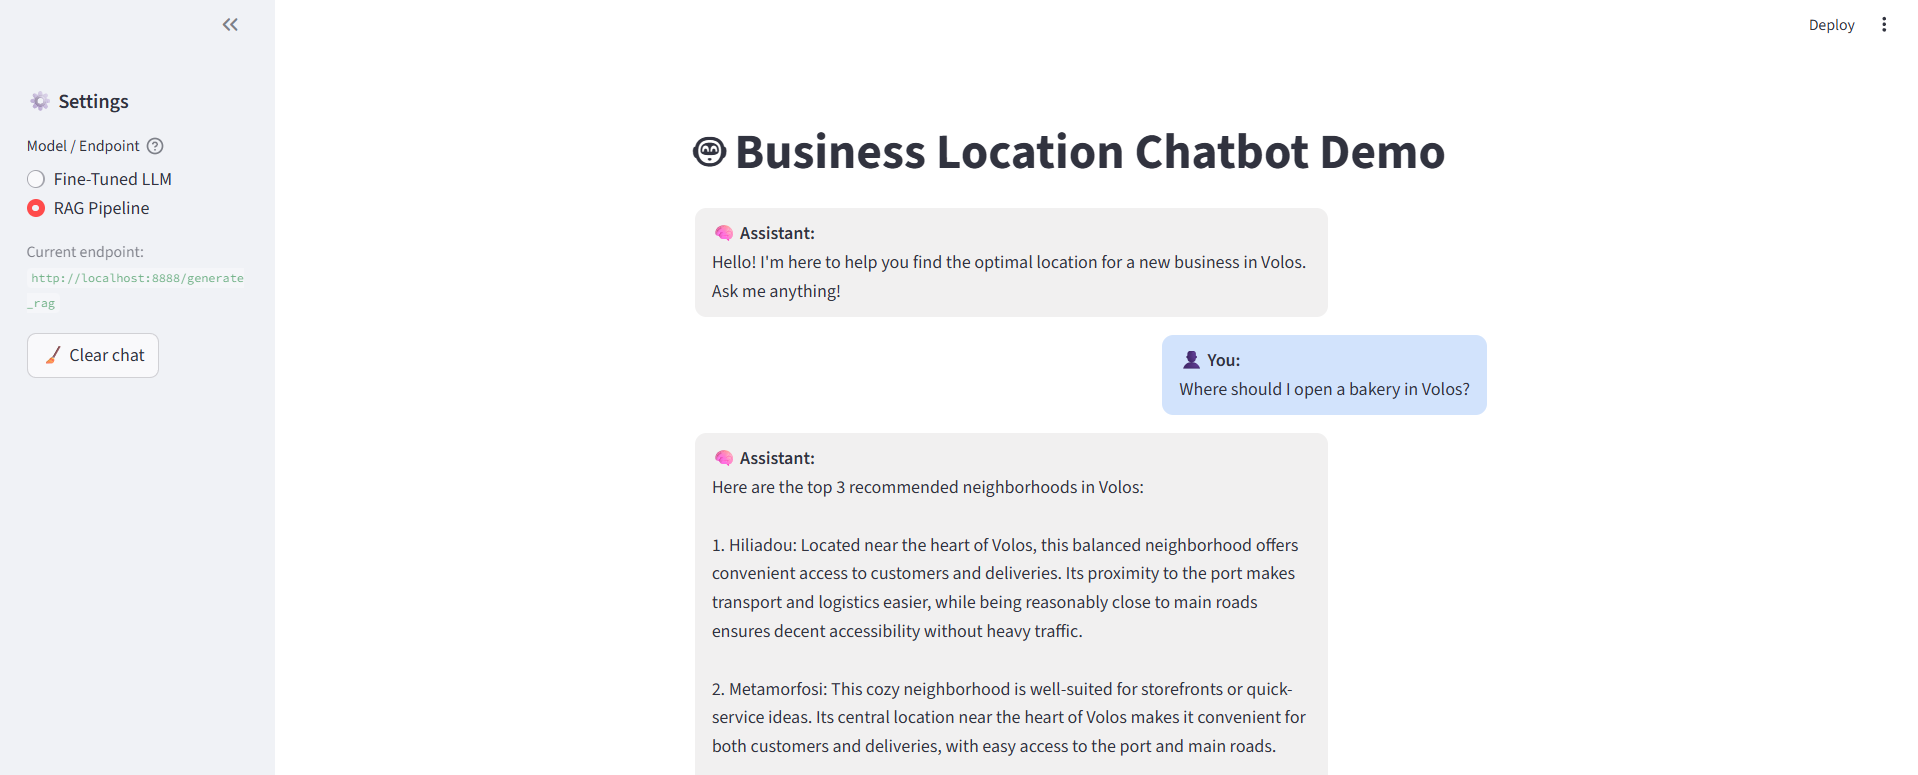
\includegraphics[width=0.8\textwidth]{figures/inf_chatbot_rag_1.png}\\[0.5em]
    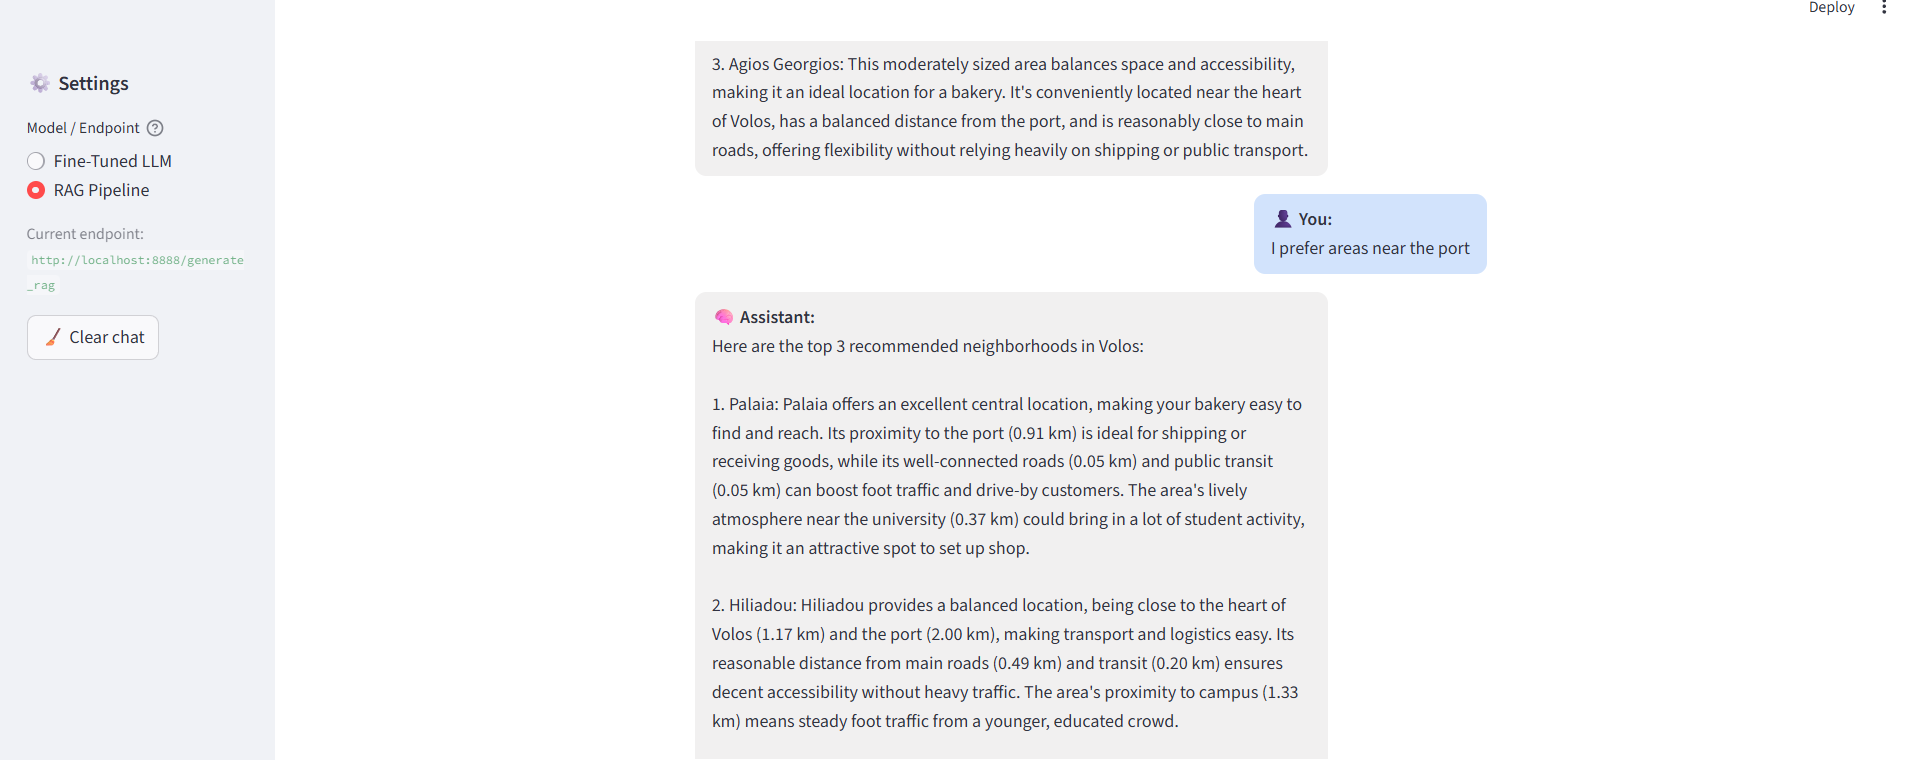
\includegraphics[width=0.8\textwidth]{figures/inf_chatbot_rag_2.png}
    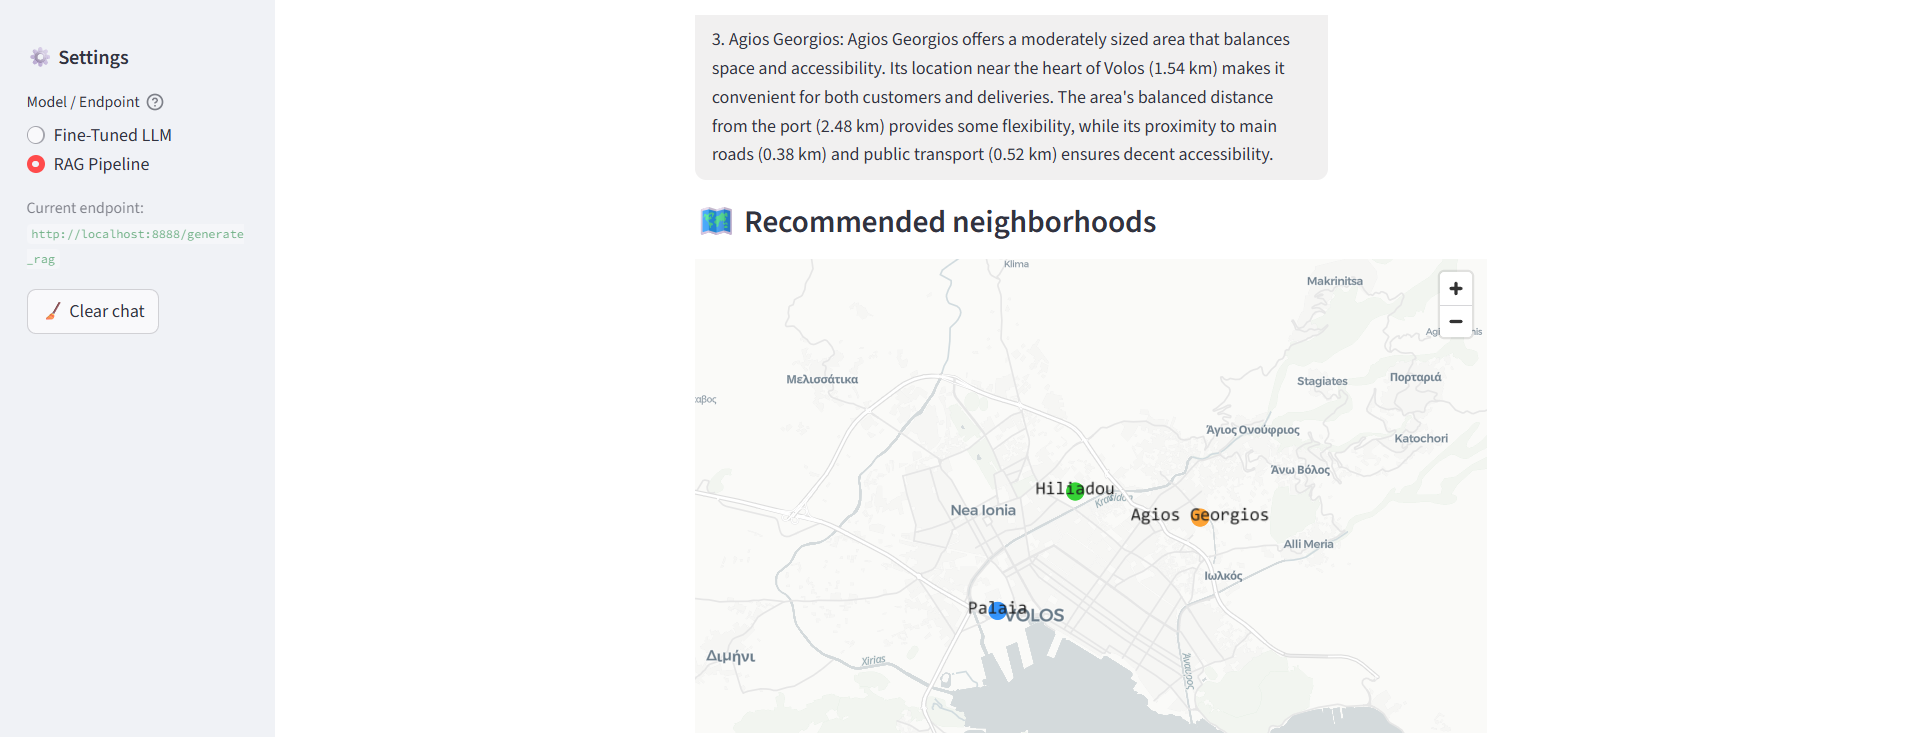
\includegraphics[width=0.8\textwidth]{figures/inf_chatbot_rag_3.png}
    
\includegraphics[width=0.8\textwidth]{figures/inf_chatbot_rag_4.png}
    \caption{Chatbot Inference - RAG Pipeline Approach}
    \label{fig:chatbot_inf_rag}
\end{figure}